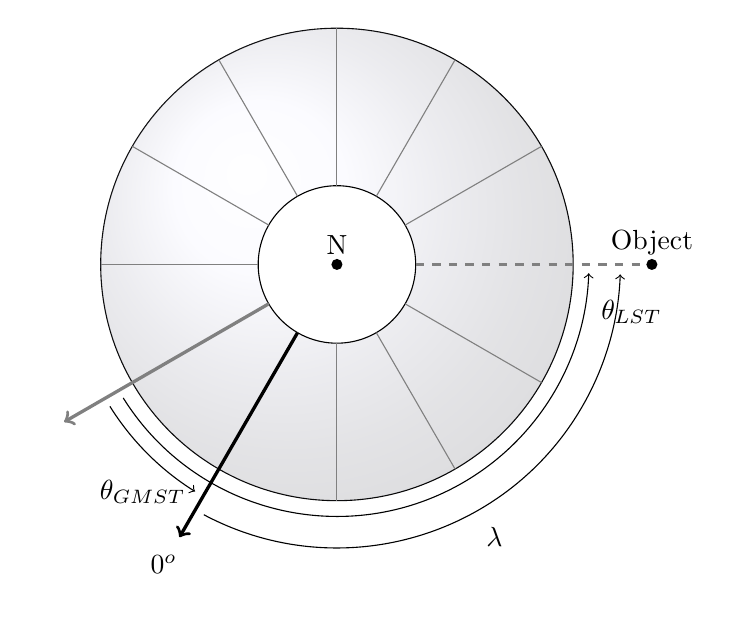
\begin{tikzpicture}

\tikzset{
	partial ellipse/.style args={#1:#2:#3}{
		insert path={+ (#1:#3) arc (#1:#2:#3)}
	}
}

\setlength{\unitlength}{1cm};
\def\ri{1};
\def\ro{3};

\draw [](0,0) circle [radius=3cm];
\shade[ball color=blue!10!white,opacity=0.20] (0,0) circle (3cm);
\filldraw[draw=black,fill=white](0,0) circle [radius=1cm];

\fill (0,0) circle[radius=2pt] node[above, align = center]{N};

\foreach \ang in {1,...,11} {
	\draw [gray] (\ang * 180 / 6:1) -- (\ang * 180 / 6:3);
}

\draw[very thick,->] (8*180/6:1) -- (8*180 / 6 : 4) 
nodeat (8 * 180 / 6:4.4){$0^o$};

\draw[gray, very thick,->] (7*180/6:1) -- (7*180 / 6 : 4) 
nodeat (7*180 / 6:4.4){\aries};

\draw (0,0) [partial ellipse=212:238:3.4cm, ->] node[left]{$\theta_{GMST}$};
\draw (0,0) [partial ellipse=212:358:3.2cm, ->] node[below = 14, right = 1]{\textbf{$\theta_{LST}$}};

\draw (0,0) [partial ellipse=242:358:3.6cm, ->] node [fill=white] at (10 * 180 / 6:4){$\lambda$};

\draw[dashed, gray, thick] (0/6:1) -- (0 / 6 : 4);
\fill (4,0) circle[radius=2pt] node[above]{Object};

\end{tikzpicture}